\section{Performance Results}

We evaluate our framework on 2 systems:
(1) Nvidia Pascal nodes with 2 socket, 14 core Intel(R) Xeon(R) CPU E5-2680
v4 @ 2.40GHz, with 2 Quadro P100-12GB; and
(2) Nvidia Volta nodes with 2 socket, 20 core Intel(R) Xeon(R) CPU E5-2698
v4 @ 2.20GHz, with 8 Tesla V100-SXM2-16GB.
Both systems use CUDA 9.0 and cuDNN 7.0.
% which are the most recent versions available on our HPC cluster.

We report results for 9 TC functions ranging from a simple matrix
multiplication kernel to a full WaveNet cell~\cite{WaveNet}. The
individual benchmarks are described below: \figref{benchmarks} and
\figref{wavenet} show the complete source code. The matrix
multiplication and convolution kernels were selected for their
dominance of the training and inference time of the most classical
networks \cite{Awan:2017:IPC:3146347.3146356,ResNext}. The other
kernels bring interesting computation patterns to enable
expressiveness and performance comparisons in more diverse network
architectures.

These results are all based on TC commit
\texttt{2e1a0dc54850} % 163fc59ac2f8bc51e9decf531b6c
available at \\
\url{https://github.com/nicolasvasilache/TensorComprehensions}.

Running the autotuner for 25 generations of 100 candidates, the
(parallel) autotuning process takes up to 1h on the longest running
kernels, and 6h in total.\footnote{Classical strategies exist to
  accelerate autotuning, such as predictive modeling and search space
  pruning \cite{Agakov:2006:UML:1121992.1122412}, but this was not the
  focus of this paper.}

\begin{figure}[h!tb]
\begin{tclisting_small}
def tmm(float(M,K) A, float(N,K) B) -> (C) { C(m,n) +=! A(m,r_k) * B(n,r_k) }
def tbmm(float(B,N,M) X, float(B,K,M) Y) -> (Z) { Z(b,n,k) +=! X(b,n,r_m) * Y(b,k,r_m) }

def 1LUT(float(E1,D) LUT1, int(B,L1) I1) -> (O1) { O1(i,j) +=! LUT1(I1(i,r_k),j) }
def 2LUT(float(E1,D) LUT1, int(B,L1) I1, float(E1,D) LUT1, int(B,L1) I1) -> (O1, O2) {
  O1(i,j) +=! LUT1(I1(i,r_k),j)
  O2(i,j) +=! LUT2(I2(i,r_k),j)
}

def MLP3(float(B,M) I, float(O,N) W2, float(O) B2, float(P,O) W3, float(P) B3, float(Q,P) W4,
	 float(Q) B4) -> (O1,O2,O3,O4) {
  O2(b,o)  = B2(o)
  O2(b,o) += O1(b,r_n) * W2(o,r_n)
  O2(b,o)  = fmaxf(O2(b,o), 0)
  O3(b,p)  = B3(p)
  O3(b,p) += O2(b,r_o) * W3(p,r_o)
  O3(b,p)  = fmaxf(O3(b,p), 0)
  O4(b,q)  = B4(q)
  O4(b,q) += O3(b,r_p) * W4(q,r_p)
  O4(b,q)  = fmaxf(O4(b,q), 0)
}

def kronecker3(float(D0,N0) W0, float(D1,N1) W1, float(D2,N2) W2, float(M,N0,N1,N2) X) -> (Y,XW1,XW2) {
  XW2(m,n0,n1,d2) +=!   X(m,n0,n1,r_n2) * W2(d2,r_n2)
  XW1(m,n0,d1,d2) +=! XW2(m,n0,r_n1,d2) * W1(d1,r_n1)
    Y(m,d0,d1,d2) +=! XW1(m,r_n0,d1,d2) * W0(d0,r_n0)
}

def group_convolution(float(N,G,C,H,W) I, float(G,F,C,KH,KW) W1, float(M) B) -> (O) {
  O(n,g,o,h,w)  = O(n,g,o,h,w) + B(m)
  O(n,g,o,h,w) += I(n,g,r_i, h + r_kh, w + r_kw) * W1(g,o,r_i,r_kh,r_kw)
}

def moments2_2d_1D(float(N,K) I) -> (mean,var) {
# var = E(x^2) - mean^2
  mean(n) +=! I(n,r_k)
  var(n)  +=! I(n,r_k) * I(n,r_k)
  mean(n)  =  mean(n) / K
   var(n)  =  var(n) / K - mean(n) * mean(n)
}

def group_normalization(float(N,G,D,H,W) I, float(G,D) gamma, float(G,D) beta,
			float(N,G) mean, float(N,G) var) -> (O,mean,var) {
  O(n,g,d,h,w) = gamma(g,d) * (I(n,g,d,h,w) - mean(n,g))
	       * rsqrt(var(n,g) - mean(n,g) * mean(n,g) + 1e-5) + beta(g,d)
}

def group_normalization_single_kernel(float(N,G,D,H,W) I, float(G,D) gamma,
				      float(G,D) beta) -> (O,mean,var) {
  mean(n,g) +=! I(n,g,r_d,r_h,r_w)
  var(n,g)  +=! I(n,g,r_d,r_h,r_w) * I(n,g,r_d,r_h,r_w)
  O(n,g,d,h,w) = gamma(g,d) * (I(n,g,d,h,w) - mean(n,g) / (D * H * W)) * rsqrt(var(n,g)/(D * H * W)
                 - mean(n,g)/(D * H * W) * mean(n,g)/(D * H * W) + 1e-5) + beta(g,d)
}
\end{tclisting_small}
  \vskip-1em
\caption{TC Benchmarks used in the experiments.  Evaluated sizes are available in Table~\ref{tbl:absolute}}
\label{fig:benchmarks}
\end{figure}

\begin{figure}[h!tb]
\begin{tclisting_small}
def wavenet1(float(B, RESIDUAL_C, RECEPTIVE_FIELD) Data,
             float(DILATION_C, RESIDUAL_C, 2) FilterWeight, float(DILATION_C) FilterBias,
             float(DILATION_C, RESIDUAL_C, 2) GateWeight, float(DILATION_C) GateBias,
             float(RESIDUAL_C, DILATION_C) ResWeight, float(RESIDUAL_C) ResBias,
             float(SKIP_C, DILATION_C) SkipWeight, float(SKIP_C) SkipBias,
             float(DILATION_FACTOR) Dilation)
    -> (FilterOut, GateOut, NonLin, Res, Skip) {
  FilterOut(b, dilation_c, rf)  = FilterBias(dilation_c)
    where b in 0:B, dilation_c in 0:DILATION_C, rf in 0:RECEPTIVE_FIELD
  FilterOut(b, dilation_c, rf) += Data(b, r_residual_c, rf)
      * FilterWeight(dilation_c, r_residual_c, 1) + ((rf - DILATION_FACTOR >= 0)
        ? Data(b, r_residual_c, rf - DILATION_FACTOR) * FilterWeight(dilation_c, r_residual_c, 0)
        : float(0))
      where rf in 0:RECEPTIVE_FIELD

  GateOut(b, dilation_c, rf)  = GateBias(dilation_c)
    where b in 0:B, dilation_c in 0:DILATION_C, rf in 0:RECEPTIVE_FIELD
  GateOut(b, dilation_c, rf) += Data(b, r_residual_c, rf)
      * GateWeight(dilation_c, r_residual_c, 1) + ((rf - DILATION_FACTOR >= 0)
        ? Data(b, r_residual_c, rf - DILATION_FACTOR) * GateWeight(dilation_c, r_residual_c, 0)
        : float(0))
      where rf in 0:RECEPTIVE_FIELD

  NonLin(b, dilation_c, rf)  = tanh(FilterOut(b, dilation_c, rf))
    where rf in 0:RECEPTIVE_FIELD
  NonLin(b, dilation_c, rf) *= 1 / (1 + exp(-GateOut(b, dilation_c, rf)))
    where rf in 0:RECEPTIVE_FIELD

  Res(b, residual_c, rf)  = Data(b, residual_c, rf) + ResBias(residual_c)
  Res(b, residual_c, rf) += NonLin(b, r_dilation_c, rf) * ResWeight(residual_c, r_dilation_c)

  Skip(b, skip, rf) +=! NonLin(b, r_dilation_c, rf) * SkipWeight(skip, r_dilation_c)
    where rf in 0:RECEPTIVE_FIELD
  Skip(b, skip, rf)  =  Skip(b, skip, rf) + SkipBias(skip)
    where rf in 0:RECEPTIVE_FIELD
}
\end{tclisting_small}
  \vskip-1em
\caption{Source of one full WaveNet cell}
\label{fig:wavenet}
\end{figure}

\begin{figure}[h!tb]
  \center  
  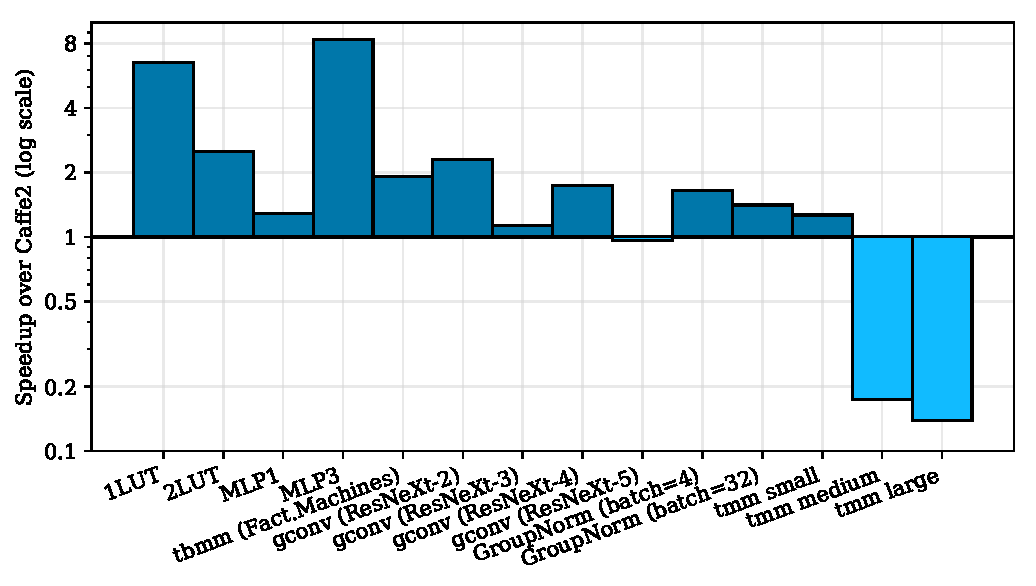
\includegraphics[width=8cm]{extra/tc_p100_caffe2_p100}
  \vskip-1.5em
  \caption{Speedup of TC-generated kernels over Caffe2 hand-tuned kernels on Quadro P100-12GB}
  \label{fig:pairwise_p100}

  \center
  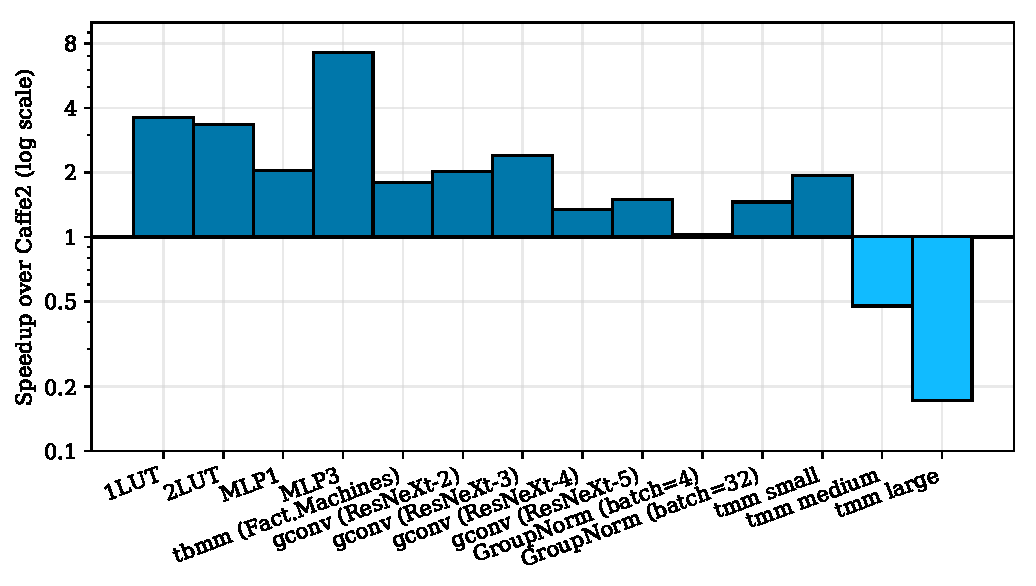
\includegraphics[width=8cm]{extra/tc_v100_caffe2_v100}
  \vskip-1.5em
  \caption{Speedup of TC-generated kernels over Caffe2 hand-tuned kernels on Tesla V100-SXM2-16GB}
  \label{fig:pairwise_v100}

  \center
  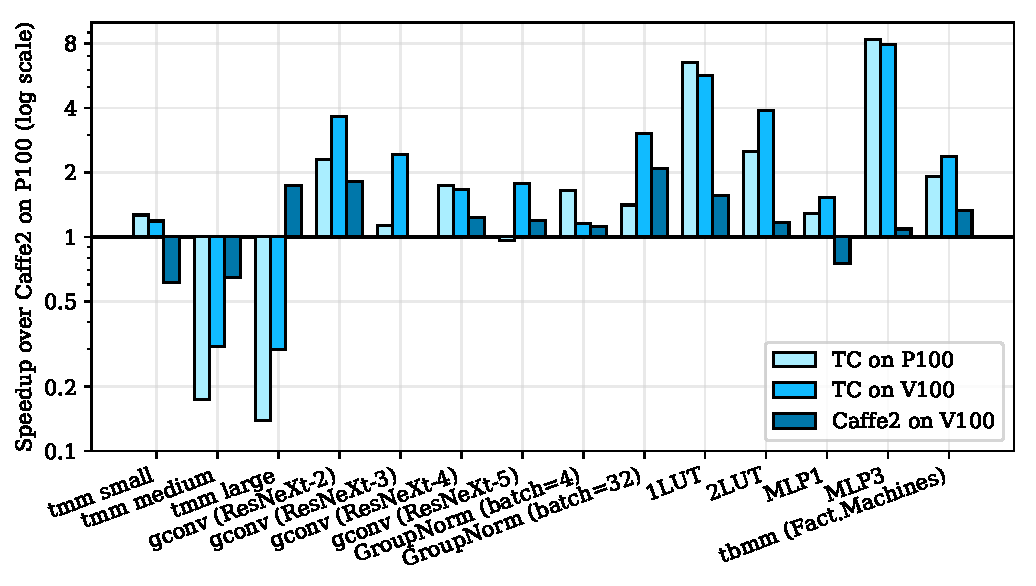
\includegraphics[width=9cm,keepaspectratio]{extra/v100_all.pdf}
  \vskip-1.5em
  \caption{\label{fig:perf}Relative performance: baseline is Caffe2
    performance on a P100 GPU}
\end{figure}

The relative performance of kernels automatically generated with TC compared to
Caffe2
is shown in \figref{pairwise_p100} and \figref{pairwise_v100}.%
\footnote{We compile Caffe2 and PyTorch from source
  (commit \texttt{6223bfdb1d32}) and integrate it in the TC testing flow
  for proper benchmarking.}
%Caffe2 is one of the fastest ML
%frameworks available and has enjoyed a close collaboration between Facebook
%and Nvidia with more than 100 contributors.
%Caffe2 efficiently wraps cuBLAS, CUB and cuDNN where relevant and provides its
%own CUDA implementations when libraries fall short.
Caffe2 provides a very strong baseline by wrapping tuned implementations, which
originate from either hand-tuned libraries or other high-performance code
generators.\footnote{A recent unification effort~\cite{F82018} made Caffe2 the
backend for PyTorch~1.0.}
\emph{We chose to compare against Caffe2 rather than against other optimization
flows due to expressivity and automation limitations}: XLA or Glow do not
support custom layers, and Halide or TVM lack range inference and automatic
parallelism discovery, which significantly complicates the expression of new
layers such as KRU and WaveNet.  The common set of comparable layers would be
limited to matrix multiplications and convolutions, while one of the main
contributions of TC is to enable exploration of new unconventional layers
\emph{before super-optimized implementations are available}.

In addition, \figref{perf} brings together the performance of TC-compiled kernels on both GPU systems, normalized to Caffe2 on P100.
This consolidated graph conveys 3 classes of information in a
common context: (1) speedup of Caffe2 V100 over Caffe2 P100 to illustrate the
out-of-the-box benefits (or lack thereof) of a faster GPU; (2) speedup of TC over Caffe2 on
P100 (main comparison); and (3) speedup of TC V100 over Caffe2
P100. The last choice may seem surprising, but presented in the context
of the other two,
allows for relative comparisons: the height of the Caffe2 V100 and TC
V100 captures the raw speedups of TC on V100.
% Alex removed "better mental model" here; until further advances, we cannot
% control the mental model of the reader...
\emph{We aim at compactly illustrating that TC provides a path to
  performance portability, improving on state of the
  art frameworks and library primitives}.

\tblref{absolute} provides absolute runtime running TC and Caffe2; all values are reported in $\mu s$.

\begin{table*}[h!tb]
{\footnotesize% 1LUT TC     Caffe2
\renewcommand{\arraystretch}{.5}
\begin{tabular}{llrrrrrr}
\toprule
	      &  &  & {\textbf{Pascal}} &  &  & {\textbf{Volta}} & \\
\textbf{1LUT} &  & p0 & p50 & p90 & p0 & p50 & p90\\
\midrule
\multirow{2}{*}{$B = 128, D = 64, E1 = 10^7, L1 = 50$}
  & TC     & 13 & 14 & 14 & 15 & 16 & 17\\
  & Caffe2 & 85 & 91 & 95 & 56 & 58 & 63\\

% 2LUT TC     Caffe2
\toprule
\textbf{2LUT} &  & p0 & p50 & p90 & p0 & p50 & p90\\
\midrule
\multirow{2}{*}{
$B = 128, D = 64, E1, E2 = 10^7, L1, L2 = 50$}
  & TC     & 52 & 54 & 57 & 35 & 35 & 37\\
  & Caffe2 & 132 & 136 & 144 & 115 & 117 & 124\\

% MLP1 TC     Caffe2
\toprule
\textbf{MLP1} &  & p0 & p50 & p90 & p0 & p50 & p90\\
\midrule
\multirow{2}{*}{$B = 128, M = 2000, N = 128$}
  & TC     & 68 & 69 & 71 & 57 & 58 & 59\\
  & Caffe2 & 87 & 89 & 91 & 116 & 118 & 123\\

% MLP3 TC     Caffe2
\toprule
\textbf{MLP3} &  & p0 & p50 & p90 & p0 & p50 & p90\\
\midrule
\multirow{2}{*}{$B = 128, N = 128, O = 64, P = 32, Q = 2$}
  & TC     & 18 & 19 & 19 & 20 & 20 & 21\\
  & Caffe2 & 157 & 159 & 169 & 144 & 146 & 164\\

% BatchMatMul TC     Caffe2
\toprule
\textbf{tbmm} &  & p0 & p50 & p90 & p0 & p50 & p90\\
\midrule
\multirow{2}{*}{$B = 500, K = 26, M = 72, N = 26$}
  & TC     & 52 & 53 & 54 & 42 & 43 & 43\\
  & Caffe2 & 94 & 102 & 103 & 76 & 77 & 78\\

% GroupConvolution TC     Caffe2
\toprule
\textbf{Group Convolution} &  & p0 & p50 & p90 & p0 & p50 & p90\\
\midrule
$C, F = 4, G, N = 32, H = 56, \textit{KH}, \textit{KW} = 3,$ & TC      & 696 & 701 & 704 & 435 & 440 & 443\\
$W = 56$                                                     & Caffe2  & 1590 & 1609 & 1621 & 879 & 888 & 896\\
\midrule
$C, F = 8, G, N = 32, H = 28, \textit{KH}, \textit{KW} = 3,$ & TC      & 574 & 576 & 578 & 269 & 270 & 272\\
$W = 28$                                                     & Caffe2  & 640 & 653 & 692 & 613 & 650 & 660\\
\midrule
$C, F = 16, G, N = 32, H = 14, \textit{KH}, \textit{KW} = 3,$ & TC     & 265 & 272 & 276 & 274 & 284 & 287\\
$W = 14$                                                      & Caffe2 & 440 & 474 & 510 & 377 & 383 & 397\\
\midrule
$C, F = 32, G, N = 32, H = 7, \textit{KH}, \textit{KW} = 3,$ & TC       & 463 & 481 & 491 & 259 & 260 & 264\\
$W = 7$                                                      & Caffe2   & 456 & 461 & 469 & 367 & 388 & 394\\

% GroupNormalization TC     Caffe2
\toprule
\textbf{Group Normalization} &  & p0 & p50 & p90 & p0 & p50 & p90\\
\midrule
\multirow{2}{*}{$C = 512, G = 32, H = 12, N = 4, W = 12$}
  & TC      & 22 & 23 & 24 & 32 & 33 & 35\\
  & Caffe2  & 37 & 38 & 40 & 33 & 34 & 35\\
\midrule
\multirow{2}{*}{$C = 512, G = 32, H = 48, N = 32, W = 48$}
  & TC     & 1285 & 1290 & 1294 & 593 & 597 & 601\\
  & Caffe2 & 1814 & 1819 & 1823 & 865 & 869 & 871\\

% TransposedMatMul TC     Caffe2
\toprule
\textbf{tmm} &  & p0 & p50 & p90 & p0 & p50 & p90\\
\midrule
\multirow{2}{*}{$K = 32, M = 128, N = 256$}
  & TC     & 15 & 15 & 15 & 15 & 16 & 17\\
  & Caffe2 & 18 & 19 & 20 & 31 & 31 & 32\\
\midrule
\multirow{2}{*}{$K = 1024, M = 128, N = 1024$}
  & TC     & 318 & 334 & 344 & 181 & 189 & 192\\
  & Caffe2 & 55 & 58 & 64 & 89 & 90 & 91\\
\midrule
\multirow{2}{*}{$K = 4096, M = 128, N = 16384$}
  & TC     & 17168 & 17209 & 17270 & 7937 & 8004 & 8096\\
  & Caffe2 & 2254 & 2388 & 2590 & 1360 & 1378 & 1419\\
\bottomrule
\end{tabular}

}
\caption{Absolute run time in $\mu s$}
\label{tbl:absolute}
\vskip-.5cm
\end{table*}

\paragraph{TMM: Transposed Matrix-Multiplication}
On matrix multiplications of shapes and sizes relevant to deep learning
workloads (i.e., small $128\times 32\times 256$,
medium $128\times 1024\times 1024$ and large $128\times 4096\times 16384$), TC
does not perform competitively, except in the low-latency small case. This is
due to: (1) the lack of a target-specific register blocking optimization, making
kernels bound by shared memory bandwidth which is an order of magnitude slower
than register bandwidth; (2) the lack of target-specific, basic-block level optimizations including careful register allocation and instruction scheduling. Matrix multiplication is the most tuned
computation kernel in history: the missing optimizations are all well known, and
may be found in use cases and open source implementations such like
CUTLASS~\cite{CUTLASS}. Alternatively, polyhedral compilation has been shown to match or outperform cuBLAS, provided sufficient target- and operator-specific information has been captured in the optimization heuristic and code generator \cite{Elango:2018:DDL:3211346.3211354}. While our scientific focus was on covering a wide range of layers with TC, a production release would need to embed such operator-specific strategies as well. One strategy would be to follow the classification and heuristic steering of Kong et al.\ \cite{KongVocabulary}. Also, TC does not replace all layers: it only acts as a custom operation in a graph; one may use TC concurrently with numerical libraries as well as custom implementations provided through TVM.

\paragraph{Group Convolution}
Group convolution is expressible with 2 lines of TC. We report comparisons for
sizes relevant to the ResNext model~\cite{ResNext}. Despite not
using either register optimizations, Fourier or Winograd domain convolutions,
TC produces faster kernels than the cuDNN ones, with running times between
$250\mu$s and $750\mu$s. To check how TC fares w.r.t.\ recent advances in optimizing group convolutions, we performed an additional comparison with the
PyTorch nightly package \ic{py36_cuda9.0.176_cudnn7.1.2_1} with
\ic{torch.backends.cudnn.benchmark=True}. TC speedups range
from $-2\%$ to $8\times$. We also observe
PyTorch performance on V100 to be worse than on P100 while TC achieves
performance portability.

\paragraph{Group Normalization}
Group Normalization was recently proposed as a way to overcome limitations of
Batch Normalization at smaller batch sizes and increase parallelism
\cite{GroupNorm}. In TC,
group normalization is a 5-line function. TC performance is
roughly $30\%$ better than the hand-tuned Caffe2 implementation. Whereas Caffe2
uses 4 \emph{handwritten} CUDA kernels, we chose to write the TC version as two
separately compiled TC functions for better reuse and overall performance.
We also experimented with writing a single fused TC but performance degraded.
This is mostly due to kernels requiring substantially different grid
configurations, which makes their fusion unprofitable.  A larger, graph-level
compiler that decides on TC function granularity, informed by the TC mapper and
the autotuner is necessary to automate this decision process, but is left for
future work.

\paragraph{Production Model}
The kernels \ic{1LUT}, \ic{2LUT}, \ic{MLP1} and \ic{MLP3} are the
backbone of a low-latency production model used at scale in a large company
and correspond to (1) reductions over a large lookup table embedding (10M
rows); (2) fused reduction over 2 large lookup table embeddings (10M rows);
(3) small size Multi-Layer Perceptron (fully-connected, bias, ReLU); and
(4) very small size, 3 consecutive Multi-Layer Perceptrons.
Despite LUT sizes, this model is essentially latency-bound.
Existing libraries are often not tuned for low-latency regimes and tend to
perform poorly.

On these examples, the need for reuse and instruction-level
parallelism is dwarfed by the need to quickly load data from the memory
into registers. TC is able to adapt to the problem size, leveraging
reduction parallelism to hide memory latency.
% AC: removed, not implemented, it was only available in PPCG-based c2isl
% and promoting indirectly referenced arrays to shared memory
This results in large speedups over Caffe2 with cuBLAS 9.0.

\paragraph{Transposed Batch MatMul}
This kernel is meant as a case study to characterize performance benefits and losses in the current flow, compared with reference libraries.
For the sizes relevant to Factorization Machines~\cite{Rendle2010}, ($500
\times 26 \times 72 \times 26$), Nvidia Profiler reports
the TC autotuned
kernel taking 56$\mu$s on the Nvidia Quadro P6000 GPU (Pascal) while both Pytorch and Caffe2 resort to the specialized cuBLAS function
\texttt{maxwell\_sgemm\_128x64\_nn} that takes 87$\mu$s.
Beyond architecture mismatch indicated in the function name, a detailed
performance comparison demonstrates that TC executes 500 blocks of $26
\times 13 = 338$ threads, compared to 500 blocks of $128$ threads for cuBLAS,
reaching $81.8\%$ occupancy instead of $23.6\%$.
Additionally,
the cuBLAS kernel shows a large number of predicated-off instructions
due to the block size not matching the problem size.
Occupancy is limited by the number of registers in both
cases (11264 vs.\ 15360), but the TC version can be distributed over~5 blocks instead of~4.\footnote{Mapping to blocks of $32 \times 13$ threads to obtain full warps
results in 60$\mu$s execution time and only 4 blocks due to the higher number of
registers per block.}
TC promotes all tensors to shared memory, saturating its bandwidth, whereas arithmetic instructions are the performance limiter for cuBLAS.
Given the large occupancy metric, performance can be further increased by promoting one tensor to
registers instead, trading off lower occupancy for reduced pressure on memory bandwidth.

\paragraph{Kronecker Recurrent Units}
These have been recently proposed as a solution to drastically reduce
model sizes by replacing the weights matrix of a linear layer by a
Kronecker product of much smaller matrices~\cite{KRU17}.  In TC, a
Kronecker product of 3 matrices is easily written as shown in the
\texttt{kronecker3} function in \figref{benchmarks}.
The following table shows
the running time in $\mu s$---or out of memory (OOM)---of a large
matrix multiplication in Caffe2 and the equivalent Kronecker product
of 3 matrices.  Note that \emph{the performance difference mostly
  comes form a using a different algorithm}.  While no specialized GPU
library primitives exist for Kronecker recurrent units, TC's automatic
flow enabled rapid exploration and reaching unprecedented levels of
performance, as shown in \tblref{kruperf}.
Clearly, this benchmark deserves a deeper discussion of the space of
possible TC derivations, including memory/computation/parallelism trade-offs
falling outside the scope of this paper.
The \texttt{kronecker3} function is one such possible implementations that
performed well for the three selected matrix shapes;
it avoids redundant computation at the expense of storage
(two tensors for intermediate computations).

\paragraph{WaveNet}
WaveNet~\cite{WaveNet} is a popular model that enables generation of realistic sounding
voices as highlighted at Google I/O 2018. We encoded a full WaveNet cell
using a single TC function and compared our generated kernel
with a WaveNet layer from PyTorch. This experiment uses a batch
size of $1$, residual and dilation channels of $32$, and $256$ skip
channels.
With TC, we observe performance improvements up to $4\times$ on Volta, as shown on \tblref{wavenetperf}.

\begin{table*}[h!tb]
\begin{center}
\renewcommand{\arraystretch}{.5}
{\footnotesize
\begin{tabular}{llrrrrrr}
  \toprule
\textbf{Algorithmic exploration} & &  & \textbf{Pascal} &  &  & \textbf{Volta} & \\
\textbf{of Kronecker Recurrent Units} & & p0 & p50 & p90 & p0 & p50 & p90\\
  \midrule
& TC Kronecker                              & 272 & 280 & 285 & 200 & 206 & 212\\
$256\times 16^3\times 32^3$ & Caffe2 MatMul & 7714 & 8158 & 8216 & 4946 & 5065 & 5466\\
  \midrule
& TC Kronecker                              & 1334 & 1349 & 1365 & 998 & 1004 & 1011\\
$256\times 16^3\times 64^3$ & Caffe2 MatMul & 64499 & 64765 & 65659 & 38280 & 39307 & 39327\\
  \midrule
& TC Kronecker                                         & 4408 & 4447 & 4472 & 4794 & 4815 & 5106\\
$256\times 16^3\times 64 \times 128^2$ & Caffe2 MatMul & OOM & OOM & OOM & OOM & OOM & OOM\\

% WaveNet autotuned
  \toprule
\textbf{WaveNet Cell}& & p0 & p50 & p90 & p0 & p50 & p90\\
  \midrule
$\mathrm{receptive~field}=4K,~\mathrm{dilation}=1$ & TC & 457 & 466 & 477 & 253 & 255 & 257\\
$\mathrm{receptive~field}=4K,~\mathrm{dilation}=1$ & PyTorch & 549 & 576 & 790 & 563 & 571 & 594\\
  \midrule
$\mathrm{receptive~field}=4K,~\mathrm{dilation}=32$ & TC & 353 & 365 & 375 & 138 & 139 & 140\\
$\mathrm{receptive~field}=4K,~\mathrm{dilation}=32$ & PyTorch & 551 & 574 & 630 & 562 & 569 & 585\\
  \bottomrule
\end{tabular}
}
\end{center}
\caption{Algorithmic exploration of Kronecker Recurrent Units and optimization of a WaveNet cell}
\label{tbl:kruperf}
\label{tbl:wavenetperf}
\vskip-.5cm
\end{table*}
